\section{Implementation}
\label{socksdirect:sec:implementation}

\begin{figure}[htbp]
	\centering
	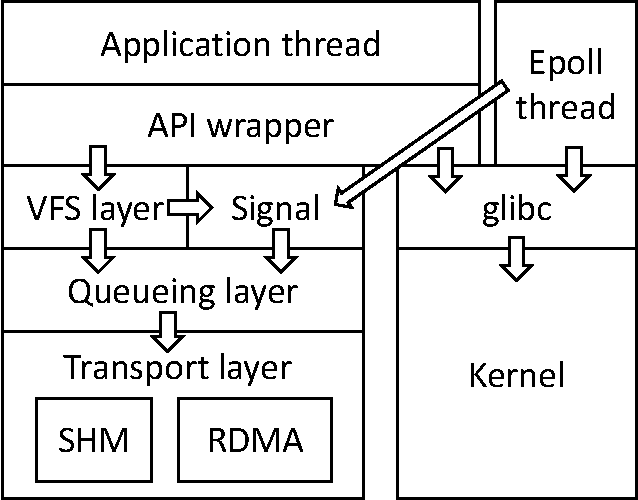
\includegraphics[width=0.25\textwidth]{images/libsd_architecture}
	
	\caption{Architecture of \libipc{}.}
	\label{socksdirect:fig:libsd-architecture}
\end{figure}


\RED{API wrapper -> file descriptor remapping layer in Figure.}

As Figure~\ref{socksdirect:fig:libsd-architecture} shows, \libipc{} has a layered structure.


%For implementation, \libipc is divided to two parts: monitor and userspace library. Both parts are implemented in $\approx$5000 lines of C/C++ code. %We take advantage of C++ templates for different types of queues in our design.



%\subsection{Seamless system call hook}
%\label{socksdirect:subsec:syscall-hook}

%\parab{LD\_PRELOAD to intercept Linux APIs.}
%\libipc uses \textit{LD\_PRELOAD} environment variable in Linux to load a shared library and intercept the system call wrappers of GNU libc.

%\parab{Multiplex file descriptor between kernel and \libipc{}.}
%Taking the idea of MegaPipe~\cite{han2012megapipe} and LOS~\cite{huang2017high}, we partition the file descriptor space between \libipc and Linux kernel. Linux assigns file descriptors from zero to $2^{30}-1$, while \libipc assigns file descriptors from $2^{31}-1$ down to $2^{30}$.

\parab{Multiplex events between kernel and \libipc{}.}
The application polls events from both sockets and other \textit{kernel file descriptors} handled by Linux kernel.
A naive way to poll kernel events is to invoke the syscall (e.g. \texttt{epoll\_wait}) every time, which incurs high overhead because event polling is a frequent operation on virtually every send and receive.
%LOS~\cite{huang2017high} periodically invokes non-blocking \texttt{epoll\_wait} syscall with kernel file descriptors, which leads to a trade-off between delay and CPU overhead. Differently,
Differently, \libipc{} creates a per-process \textit{epoll thread} which invokes \texttt{epoll\_wait} syscall to poll kernel events. Whenever epoll thread receives a kernel event, it broadcasts the event to application threads via shared memory queues. Then the signal layer in \libipc{} will return such kernel events together with user-space socket events to the application.
%Note that Linux allows an event to be received by multiple threads.

**Accelerate access to local storage.**
Use SPDK and user-mode file system (cite). How to multiplex processes in accessing a file system? (1) Directory and metadata are directed to the monitor, (2) read/write within the allocated area of a file is handled by the process itself, (3) append or read/write outside the allocated area is handled by the master process of a shared file. The monitor pre-allocates free blocks to processes (batch allocation and free).
